\chapter{Iterator pattern}

\section{Định nghĩa}
Iterator Pattern là một trong những Pattern thuộc nhóm hành vi (Behavior Pattern). Nó được sử dụng để “Cung cấp một cách thức truy cập tuần tự tới các phần tử của một đối tượng tổng hợp, mà không cần phải tạo dựng riêng các phương pháp truy cập cho đối tượng tổng hợp này”.\\

Nói cách khác, một Iterator được thiết kế cho phép xử lý nhiều loại tập hợp khác nhau bằng cách truy cập những phần tử của tập hợp với cùng một phương pháp, cùng một cách thức định sẵn, mà không cần phải hiểu rõ về những chi tiết bên trong của những tập hợp này.

\section{Mục đích sử dụng}
Nếu trong project của các bạn có quá nhiều cấu trúc dạng danh sách như cấu trúc cây, mảng, ngăn xếp, hàng đợi.... Và bạn muốn có một quy tắc chung cho chúng như đều có thêm sửa xoá chẳng hạn. Như vậy lúc này chúng ta có thể tìm tới Iterator.

\section{Mô hình cấu trúc}
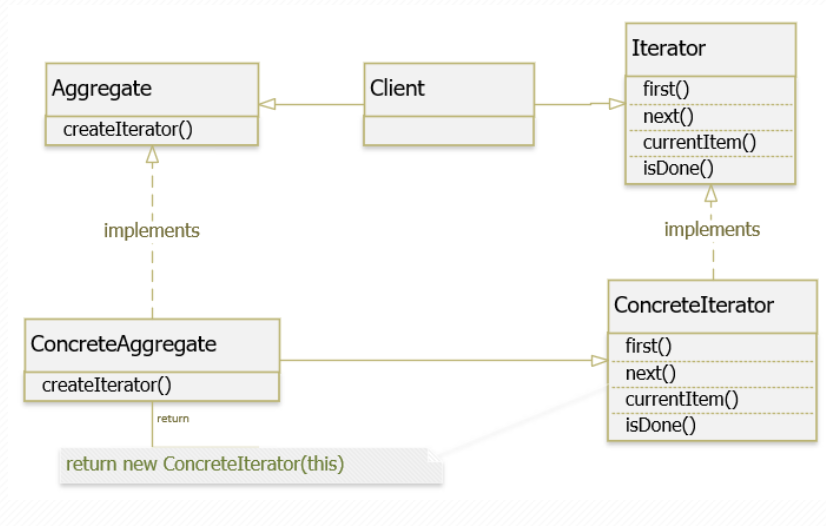
\includegraphics[width=\columnwidth]{GALLEYS/images/chapter3/diagram1}\\
\textbf{Aggregate} : là một interface định nghĩa định nghĩa các phương thức để tạo Iterator object.\\
\textbf{ConcreteAggregate} : cài đặt các phương thức của Aggregate, nó cài đặt interface tạo Iterator để trả về một thể hiện của ConcreteIterator thích hợp. \\
\textbf{Iterator} :  là một interface hay abstract class, định nghĩa các phương thức để truy cập và duyệt qua các phần tử. \\
\textbf{ConcreteIterator} :  cài đặt các phương thức của Iterator, giữ index khi duyệt qua các phần tử. \\
\textbf{Client} : đối tượng sử dụng Iterator Pattern, nó yêu cầu một iterator từ một đối tượng collection để duyệt qua các phần tử mà nó giữ. Các phương thức của iterator được sử dụng để truy xuất các phần tử từ collection theo một trình tự thích hợp.\\\\
VD cụ thể:\\
Tình huống: mô tả thực đơn cho những bữa ăn của hai cửa hàng có PancakeHouseMenu và DinnerMenu. Nhưng hai menu này được thực hiện khá là khác nhau
\newpage
\begin{multicols}{2}
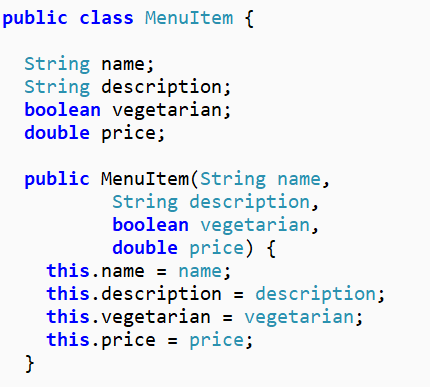
\includegraphics[width=1\columnwidth]{GALLEYS/images/chapter3/images1}\\
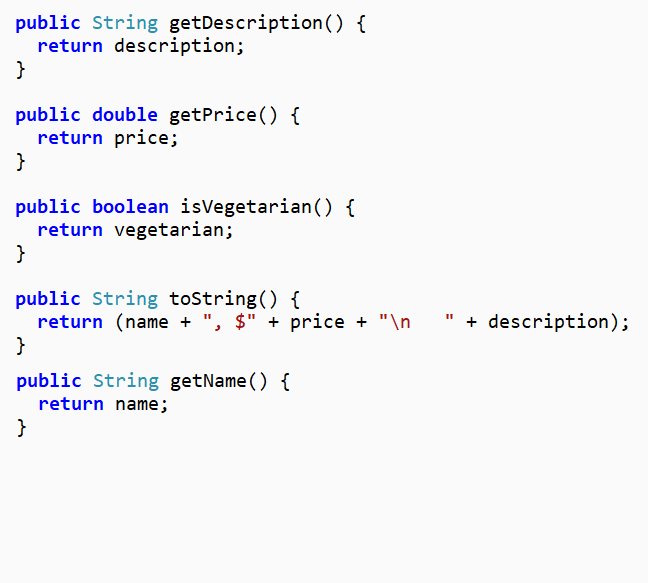
\includegraphics[width=1\columnwidth]{GALLEYS/images/chapter3/images2}
\end{multicols}
Trong class này chúng ta có những hàm cơ bản:\\
Hàm construct khởi tạo name,description,vegetarian,price
Các thuộc tính\\ name(String),description(String),vegetarian(boolean),price(double) các thuộc tính này đều có phạm vi là private.
Các hàm getter và setter cho các trường giá trị.\\

	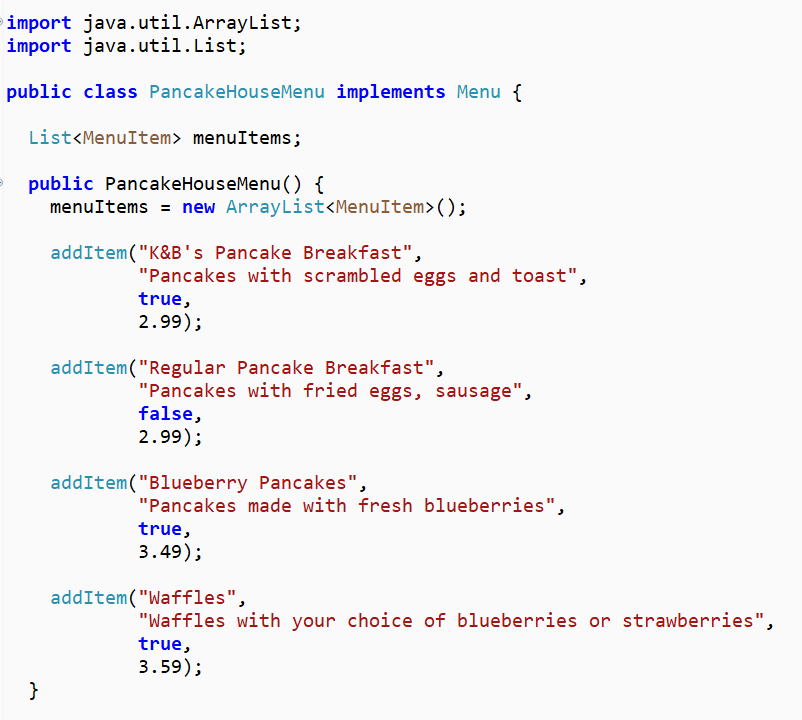
\includegraphics[width=1\columnwidth,height=0.51\textheight]{GALLEYS/images/chapter3/images3}\\
	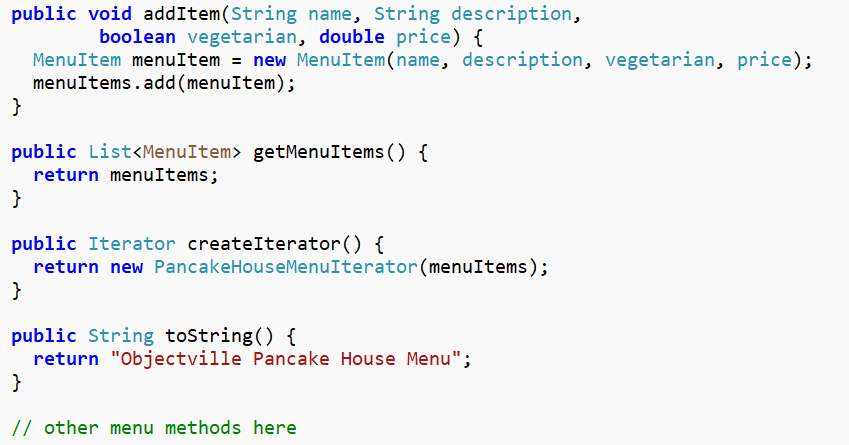
\includegraphics[width=1\columnwidth,height=0.48\textheight]{GALLEYS/images/chapter3/images4}\\\\
Tại PancakeHouseMenu:\\
- Có ArrayList<> dùng để lưu trữ dữ liệu.\\
- Trong construct của lớp mỗi menu item được thêm vào ArrayList<>, mỗi menuItem có tên, mô tả, đồ ăn chay hay không và giá tiền.\\
- Phương thức addItem() dùng để thêm menu mới vào trong ArrayList<>,
Phương thức getMenuItem dùng để trả về danh sách các menu.\\
- Phương thức createIterator() cho phép chúng ta trả về danh sách menu theo iterator pattern mà chúng ta sẽ nói rõ hơn nữa ở phía sau.\\

\begin{center}
	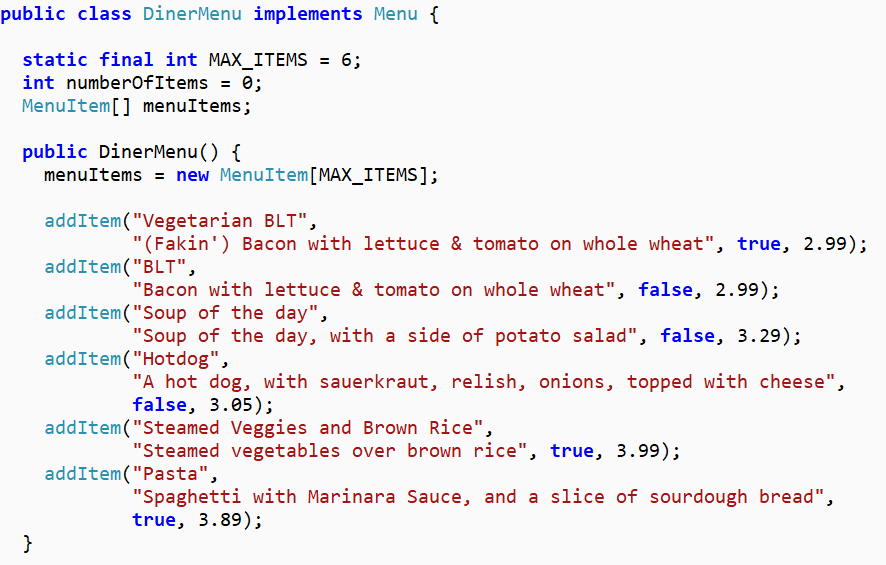
\includegraphics[width=1\columnwidth,height=0.48\textheight]{GALLEYS/images/chapter3/images5}\\
	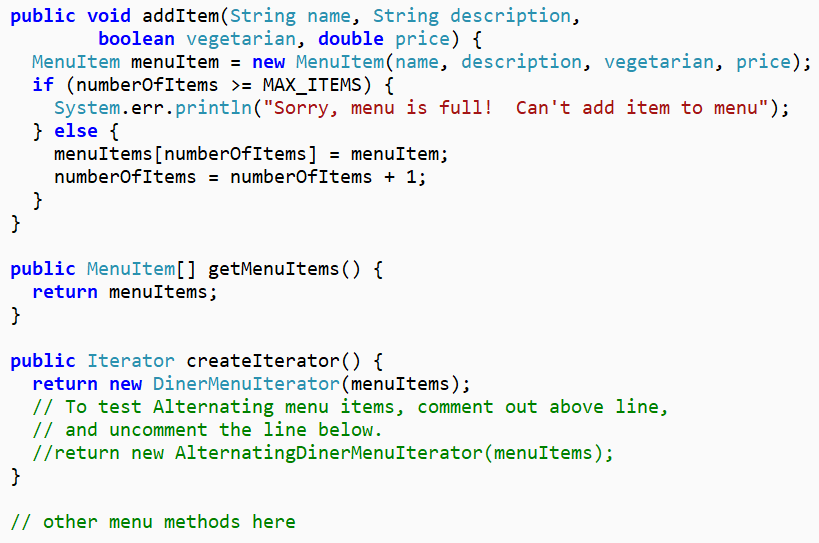
\includegraphics[width=1\columnwidth,height=0.48\textheight]{GALLEYS/images/chapter3/images6}\\
\end{center}
Trong DinnerMenu có cách thức hơi khác so với PancakeHouseMenu:\\
- Trong class này sử dụng Array thay cho ArrayList<> nhằm mục đích quản lí số lượng các menu, và lấy menu một cách đơn giản hơn.\\
- Phương thức addItem() sẽ kiểm tra nếu số lượng thực đơn đã đầy, item đó sẽ không được thêm vào mảng.\\
- Phương thức createIterator() có tác dụng tương tự như trong class PancakeHouseMenu. Đặc biệt cách thức này chúng ta sẽ chỉ biết là nó return về menuItem mà không biết nó được triển khai như thế nào.\\

 Những phương thức khác đều hoạt động tương tự như PancakeHoueMenu.Nhưng một vấn đề nảy ra: nếu muốn in ra menuItem của 2 menu này cho một nữ phục vụ (Waitress) sẽ rất là khó khăn vì cú pháp của array và arrayList khác nhau, và cữ mỗi menu thực hiện in một lần cũng mất thời gian hay là việc phân loại bữa trưa và bữa chiều của 2 menu và in ra thực đơn bữa trưa (chiều). vì thế chúng ta cần phải cho chúng implements menu chung để giảm thiểu các vòng lặp.\\
Class menu sẽ giải quyết điều đó: \\
\begin{multicols}{2}
	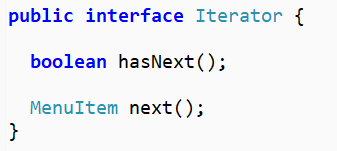
\includegraphics[width=1\columnwidth]{GALLEYS/images/chapter3/images7}
	Trong interface Iterator, có 2 phương thức gói gọn là hasNext() cho chúng ta biết có còn phần tử để duyệt qua hay không và next() trả về đối tượng tiếp theo trong tập hợp
\end{multicols}
\begin{multicols}{2}
	Giao diện interface Menu tạo ra phương thức createIterator().\\
	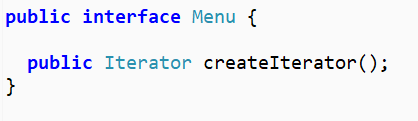
\includegraphics[width=1\columnwidth]{GALLEYS/images/chapter3/images8}
\end{multicols}
\begin{center}
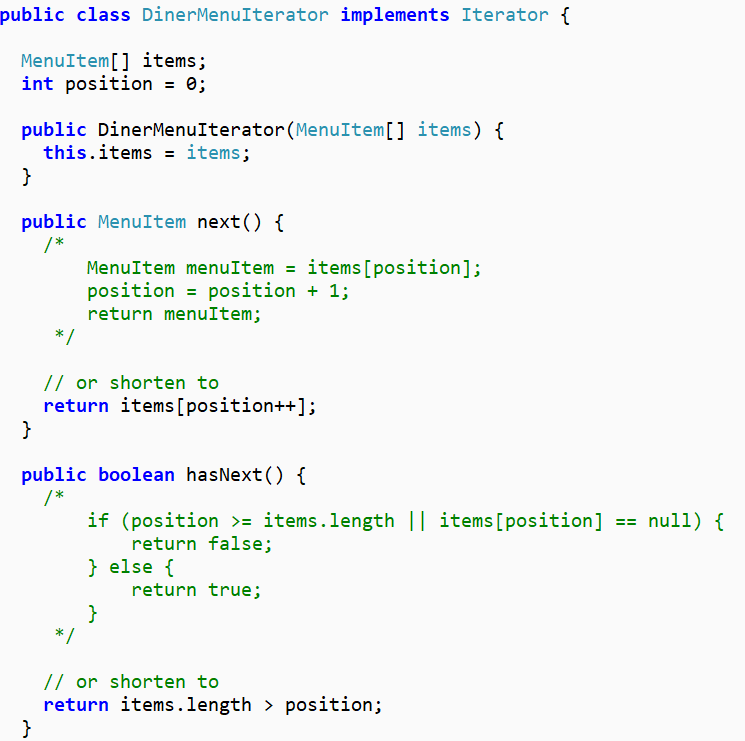
\includegraphics{GALLEYS/images/chapter3/images9}\\
\end{center}
Class này được implement từ interface Iterator.\\
Với một position dùng để duy trì vị trí lặp trên mảng . mặc định bằng 0.\\
Hàm construct lấy mảng mà chúng duyệt qua.\\
Việc cho các menu implement một interface iterator đã giúp giảm bớt độ phức tạp dành cho nữ phục vụ. \\
\begin{center}
	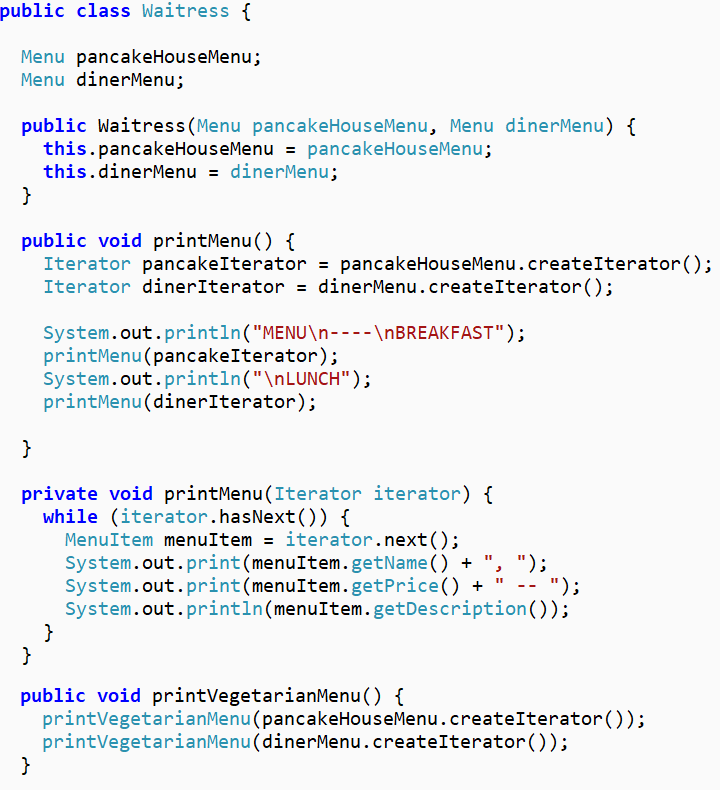
\includegraphics[width=1\columnwidth,height=0.7\textheight]{GALLEYS/images/chapter3/images10}\\
\end{center}
 Trong hàm khởi tạo của Waitress sẽ khởi tạo ra 2 menu.\\
Phương thức printMenu khởi tạo 2 Iterator.\\
Sau đó printMenu được overload với mỗi iterator.\\
Phương thức private printMenu in ra danh sách menu.\\
\begin{center}
	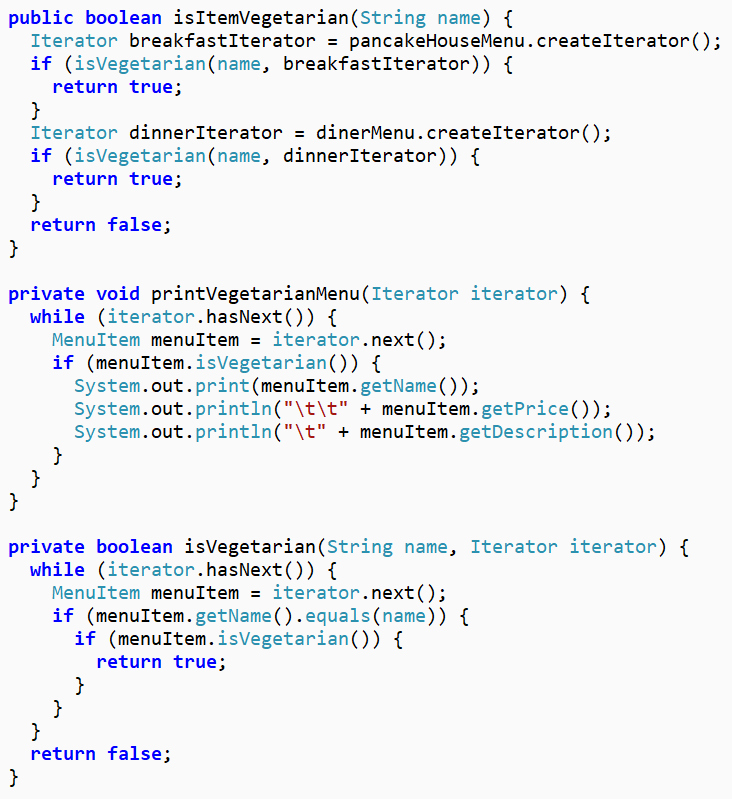
\includegraphics[width=1\columnwidth,height=0.7\textheight]{GALLEYS/images/chapter3/images11}\\
\end{center}
Tương tự chúng ta sẽ triển khai được các lớp khác.\\
Và đây là kết quả:
\begin{center}
	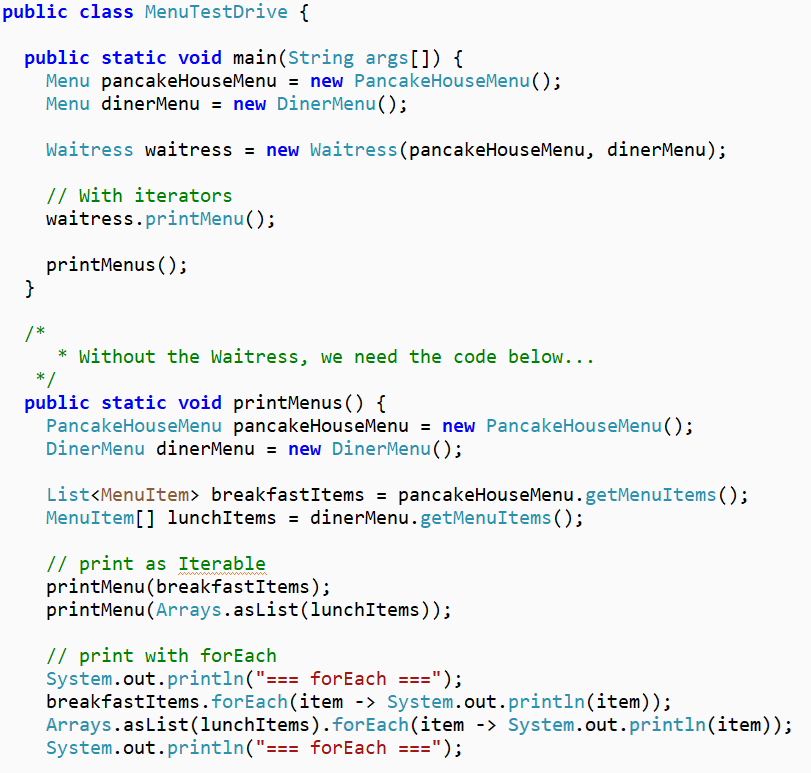
\includegraphics[width=1\columnwidth]{GALLEYS/images/chapter3/images12}\\
	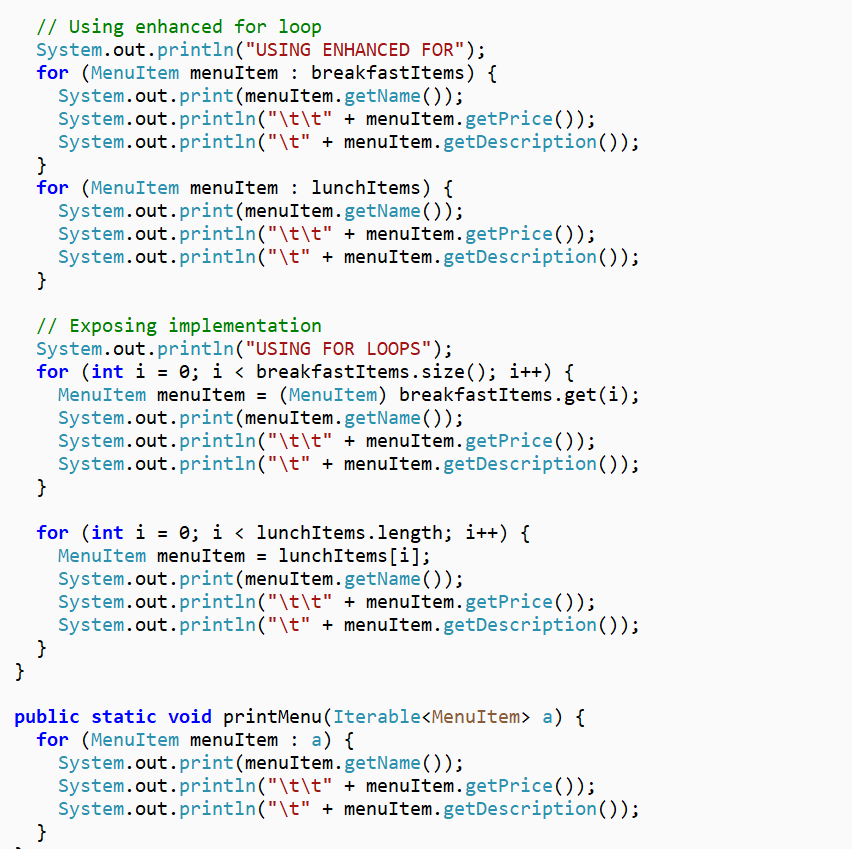
\includegraphics[width=1\columnwidth]{GALLEYS/images/chapter3/images13}\\
\end{center}
\begin{center}
	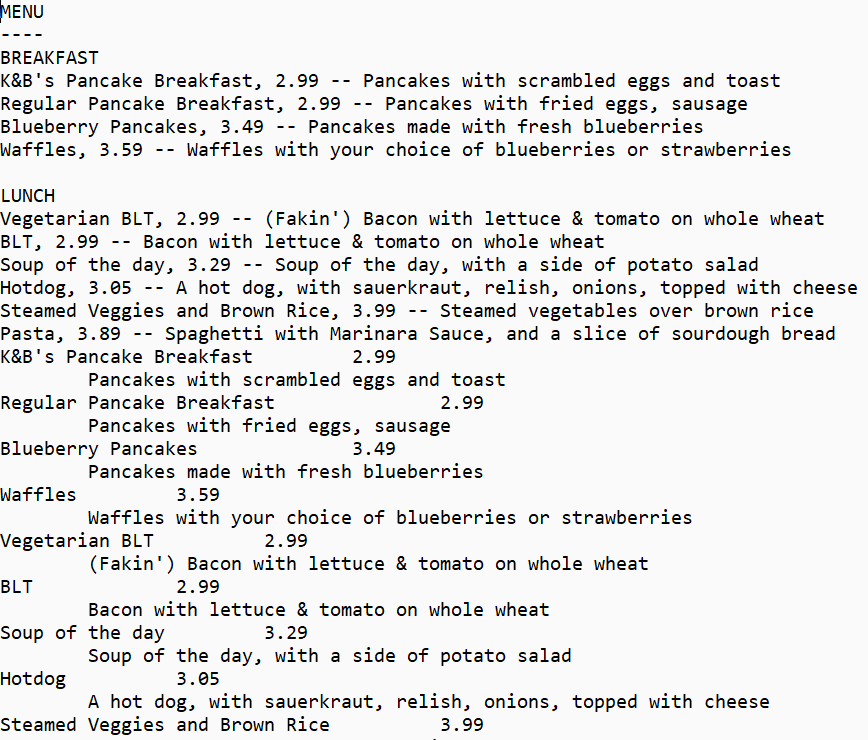
\includegraphics[width=1\columnwidth,height=0.8\textheight]{GALLEYS/images/chapter3/images14}\\
\end{center}
Đây là một phần của kết quả.\\
Như vậy Iterator pattern giúp chúng ta in ra danh sách các phần tử một cách rất đơn giản, nó là một trong những pattern được ứng dụng khá cao trong thực tế.

\section{Iterator Pattern trong thực tế}
Iterator Pattern được áp dụng khi:

\begin{itemize}
	\item Cần truy cập nội dung của đối tượng trong tập hợp mà không cần biết nội dung cài đặt bên trong nó.\\
	\item Hỗ trợ truy xuất nhiều loại tập hợp khác nhau.\\
	\item Cung cấp một interface duy nhất để duyệt qua các phần tử của một tập hợp.\\
\end{itemize}